\chapter{正态分布}
pauca sed matura
\makebox{}\hfill Carl Friedrich Gauss

\section*{学习目标}
\begin{todolist}
	\item 理解连续随机变量与离散随机变量的区别
	\item 理解正态分布常见的场景
	\item 掌握正态分布的标记手段
	\item 解释正态分布的概率图像特征,包括均值,标准差以及面积
	\item 掌握随机变量标准化的方法
	\item 能够标准正态分布表查询对应概率或者数值
	\item 说明二项分布和正态分布之间的联系,以及运用能够将两者近似的条件
	\item 利用正态分布去预估二项分布的概率
\end{todolist}
\clearpage

\section{二项分布的图像}
\label{sec:graph of binomial}
在之前的章节当中,我们更多的是利用表格来描述随机变量的分布,但是并非意味着不能用图表的方式进行表示。只不过是因为很多情况下由于其概率值是小数,用柱状图的方式不太方便而已,但是现在我们忽略这个不便,将一个二项分布的柱状图表示出来。
\begin{figure}[H]
\centering
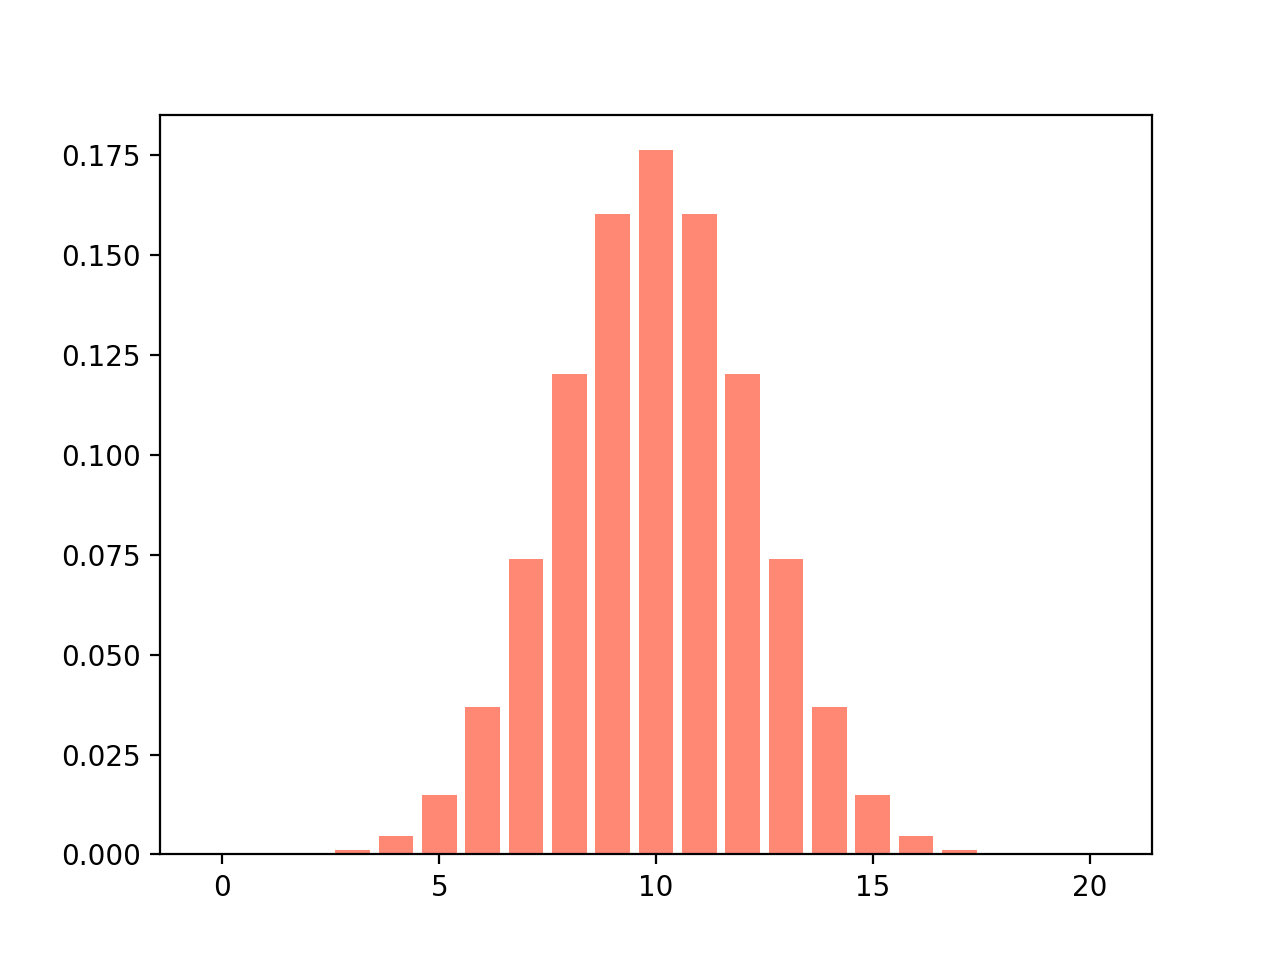
\includegraphics[width=0.8\textwidth]{binomial graph}
\label{fig:binomial graph}
\caption{$X\sim B(20,0.5)$的分布图}
\end{figure}
这张bar graph只有两个需要说道的地方,能够理解这两个有助于帮助理解正态分布。纵坐标是\gls{prob density},而不是之前所提的概率;这样操作的目的在于第二点,用概率密度乘以随机变量的跨度Step Length得到\textbf{面积},我们此时用面积来代表\textbf{概率}。举个例子,当$X=10$的时候,对应的红色bar的$X$取值为$[9.5,10.5]$\footnote{虽然X就是10,而不是9.5-10.5之间的数字},跨度为$1$。所以根据这张表格进行推导,可知$P(X=10)=0.175\times(10.5-9.5)=0.175$。

\begin{TaskBox}
1. 尝试用二项分布模型求算$P(X=10)$的精确结果\\
2. 尝试对比一下分布表格和图像的优缺点
\end{TaskBox}

因此这种表格实际上就类似于\ref{subsec:Freqeuncy Density Histogram},只不过将频率密度转变为概率密度而已。
\clearpage

\section{连续随机变量}
现在考虑如下的两个随机实验。
\begin{TaskBox}
说出一个介于1-10的正数(包括端点值);\\和在数轴当中1-10的长度上随机选择一个点;\\
\tcblower
思考一下,这两件随机实验是否是同样的实验?在这两个实验中,最终结果为2的概率是否相同?
\end{TaskBox}

这两个问题的回答都是不,因为在第一个随机实验当中,最终可能的结果数目是有限的,但是在第二个实验当中,结果是无穷无尽的。换言之,第一个的随机变量是属于经典的\emph{离散}型随机变量;而第二个随机变量是典型的\emph{连续}型随机变量。
自然导致,在前一种实验当中,结果为2的概率为$\frac{1}{10}$;在第二次实验当中,结果为2的概率为0\footnote{在这里,概率为0并不表示无法发生的不可能事件}。

按照这种角度的理解,像上一章节当中所学的二项分布,几何分布都是属于离散变量,因为产生的结果是间隔的。并不在连续随机变量的讨论当中。那么典型的连续性随机变量有什么呢?

像刚才在$[1-10]$之间随机的实数就是一种均匀的连续随机变量;再比如在一群人当中任意取一个人的身高/体重;医院里新生儿的出生体重;股市当中任意一只股票的收益率等,这些我们通常都当成连续随机变量来处理。在这里可能有学生质疑,明明身高或者体重是169cm,65.05kg这样离散的数据,怎么能说成是连续的呢?这个问题的回答是,测量精确度的问题。我身高169cm,难道不带小数点吗?小数点不可以精确到无数多位吗。所以这些场景就是经典的连续随机变量。
\clearpage

\section{正态分布}
\label{sec:Normal Distribution}
当我们收集到之前所说的体重,身高,股市收益率等一系列分布的情况的时候,形成如下图的histogram
\begin{figure}[H]
\centering
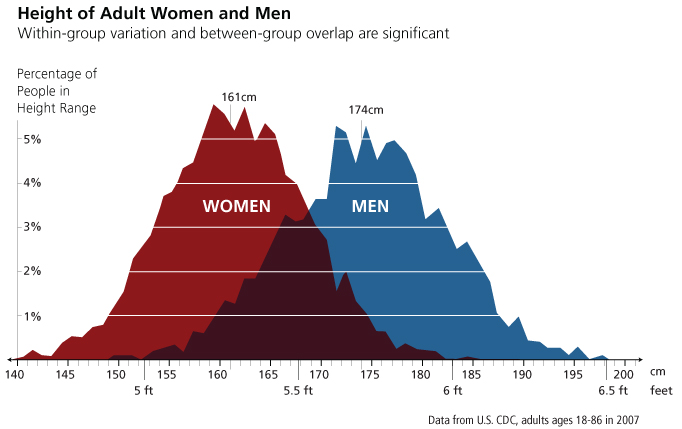
\includegraphics[width=0.3\textwidth]{height.jpg}
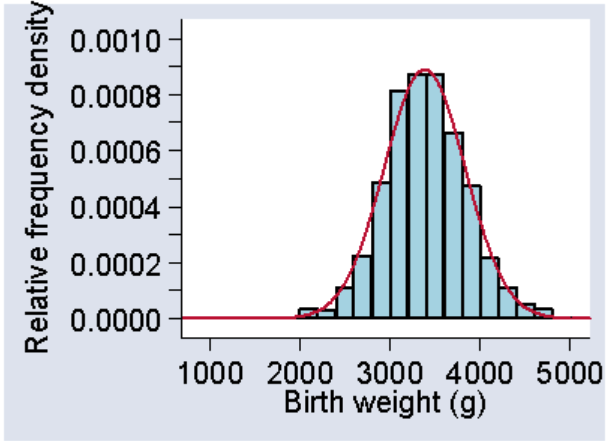
\includegraphics[width=0.3\textwidth]{birthweight.png}
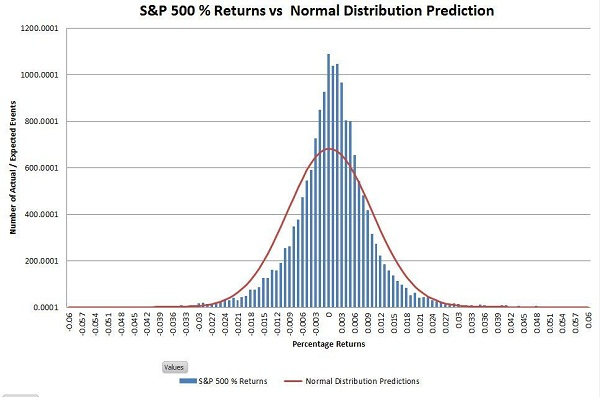
\includegraphics[width=0.3\textwidth]{stockmarket}
\end{figure}
有没有发现和之前的标准的二项分布有点像?或者后面两张图当中红色的曲线似乎统治着这些分布情况。

具有如下的特征:
\begin{itemize}
	\item 中间频率比较大,两端频率比较小,意味着取值比较极端的时候(极大,极小)频率或者说概率也不大
	\item 两端对称
\end{itemize}

而这条红色曲线就是概率学当中如雷贯耳的钟型曲线、高斯曲线,也就是正态分布或者\href{https://en.wikipedia.org/wiki/Normal_distribution}{高斯分布}的概率密度函数曲线!

\subsection*{定义和符号}
当一个随机变量$X$服从正态分布的时候,我们会标记为$X\sim N(\mu,\sigma^2)$的形式。解释其中的含义,$N$是normal distribution的缩写,$\mu$是老朋友了,代表期望,$\sigma$是标准差\footnote{其他分布是一般是求算概率结束后再求算期望和方差(标准差);但是正态分布一般是将期望和标准差作为已知条件,再求算概率}。

\subsection*{概率求算}
在求算正态分布的概率之前,有两个问题需要明确:\\

1. 正态分布能不能用Probability Distribution Table来罗列?2. 在连续随机变量当中,特定值的概率都是0,那该求算什么?

这两个的问题的回答其实早已经出现在\ref{sec:graph of binomial}和\ref{sec:Normal Distribution}中。首先,连续随机变量无法用表格的方式呈现,因为随机变量$X$的取值是无穷多且连续的。其次,虽然无法求算概率,但是可以使用图像的方式进行表示,而且可以求算概率的\emph{密度}。

因此,在正态分布的所有求算当中,我们都是采用绘制概率分布图像的方式来解决这些问题的。不过实际上,既然有图像,其实也是能够写出表达式的,高斯这个神人推导出正态分布的概率密度函数为:
\[
	\phi (x) = \frac{1}{\sqrt{2\pi}\sigma} \cdot e^{-\frac{(x-\mu)^2}{2\sigma^2}}
\]

\begin{figure}[H]
\centering
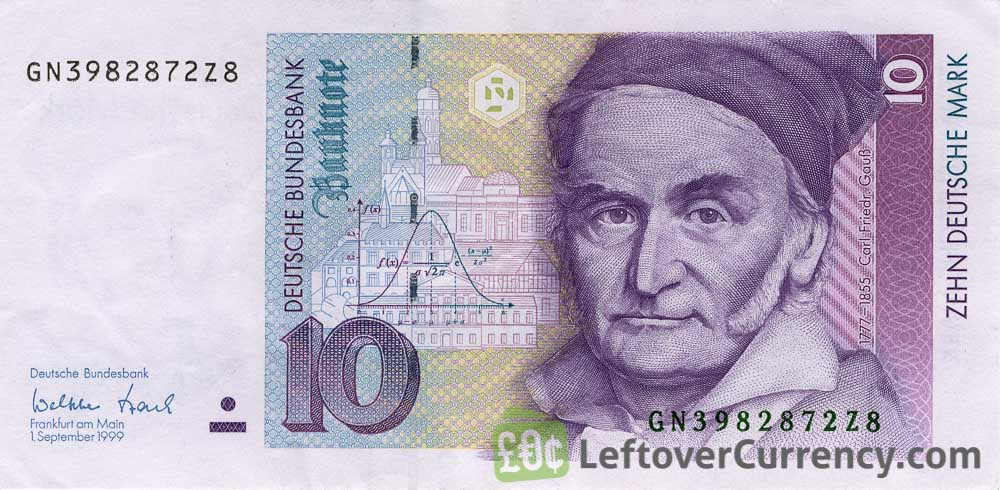
\includegraphics[width=0.8\textwidth]{currency}
\caption{德国马克10元纸币上的高斯分布}
\end{figure}

\subsubsection*{正态分布曲线}
在A-Level考试当中,并不要求掌握表达式和概率密度的求算,但是需要理解正态分布的图像,并且绘制草图即可。
因此,在这里给出$X\sim N(0,1^2)$,$X\sim N(-1,0.5^2)$和$X\sim N(3,2^2)$三种正态分布图像,可以对比一下,那一条颜色和10元纸币上的最接近。
\begin{figure}[H]
\centering
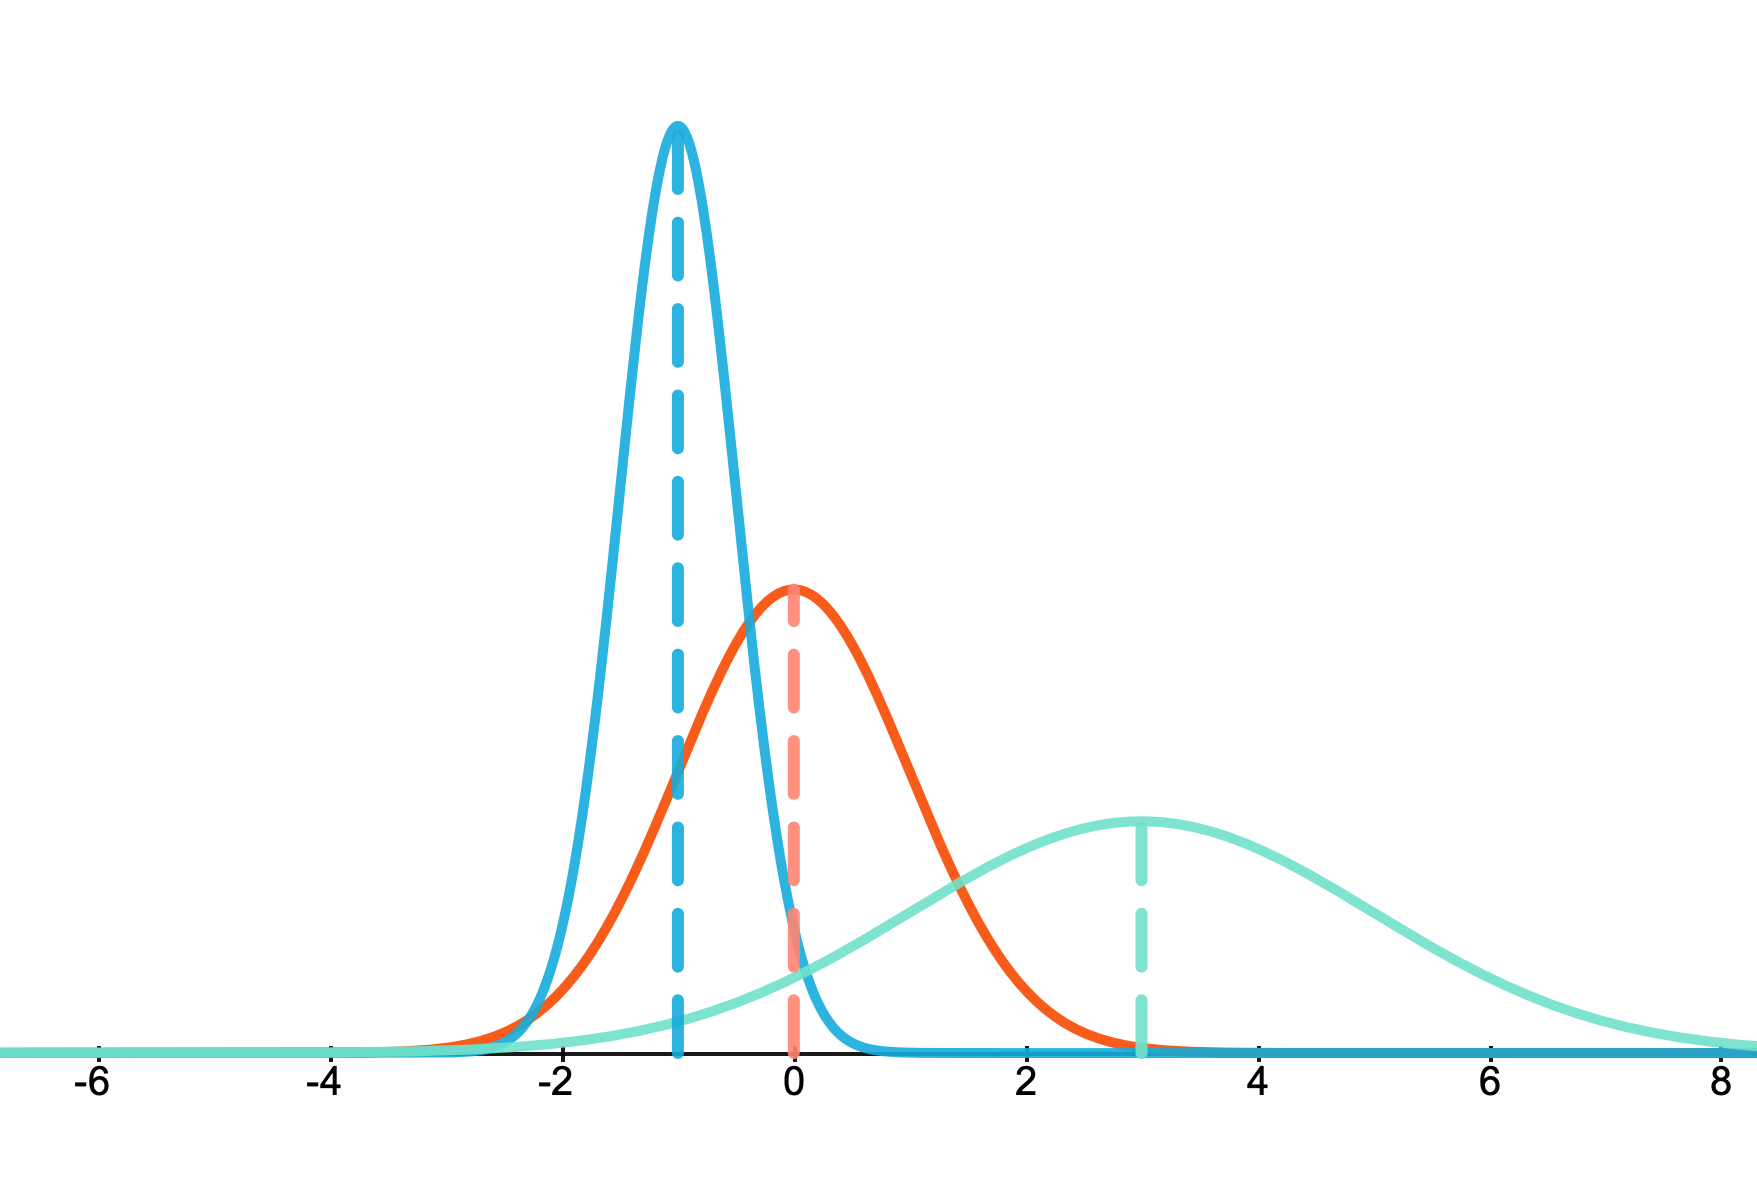
\includegraphics[width=0.8\textwidth]{bellcurve}
\caption{三种不同参数的正态分布图像}
\end{figure}
有没有发现,我们并不关注具体数值,只需要明确一下的几个特征即可:
\begin{enumerate}
	\item 所有的正态分布都是对称的分布
	\item 对称轴所在的值为该分布的期望
	\item 图像呈高峰细尾的状态,类似一座山或者大钟
	\item 如果\emph{标准差}越大,则随机变量的分布更加集中(底部跨度比较小),体现在峰更高,尾部更低。
	\item 函数图像下方包围的面积为$1$
\end{enumerate}
还记得\ref{sec:graph of binomial}中提到,用bar的面积来代表概率吗?沿用这个思路,此时虽然没有bar,但是依旧可以沿用这个思路,人为绘制$X=x_1$和$X=x_2$这两个竖线,与正态分布的曲线组合形成一个`梯形',该梯形的面积就是就是随机变量取值介于$[x_1,x_2]$的概率,如下图所示:
\begin{figure}[H]
\centering
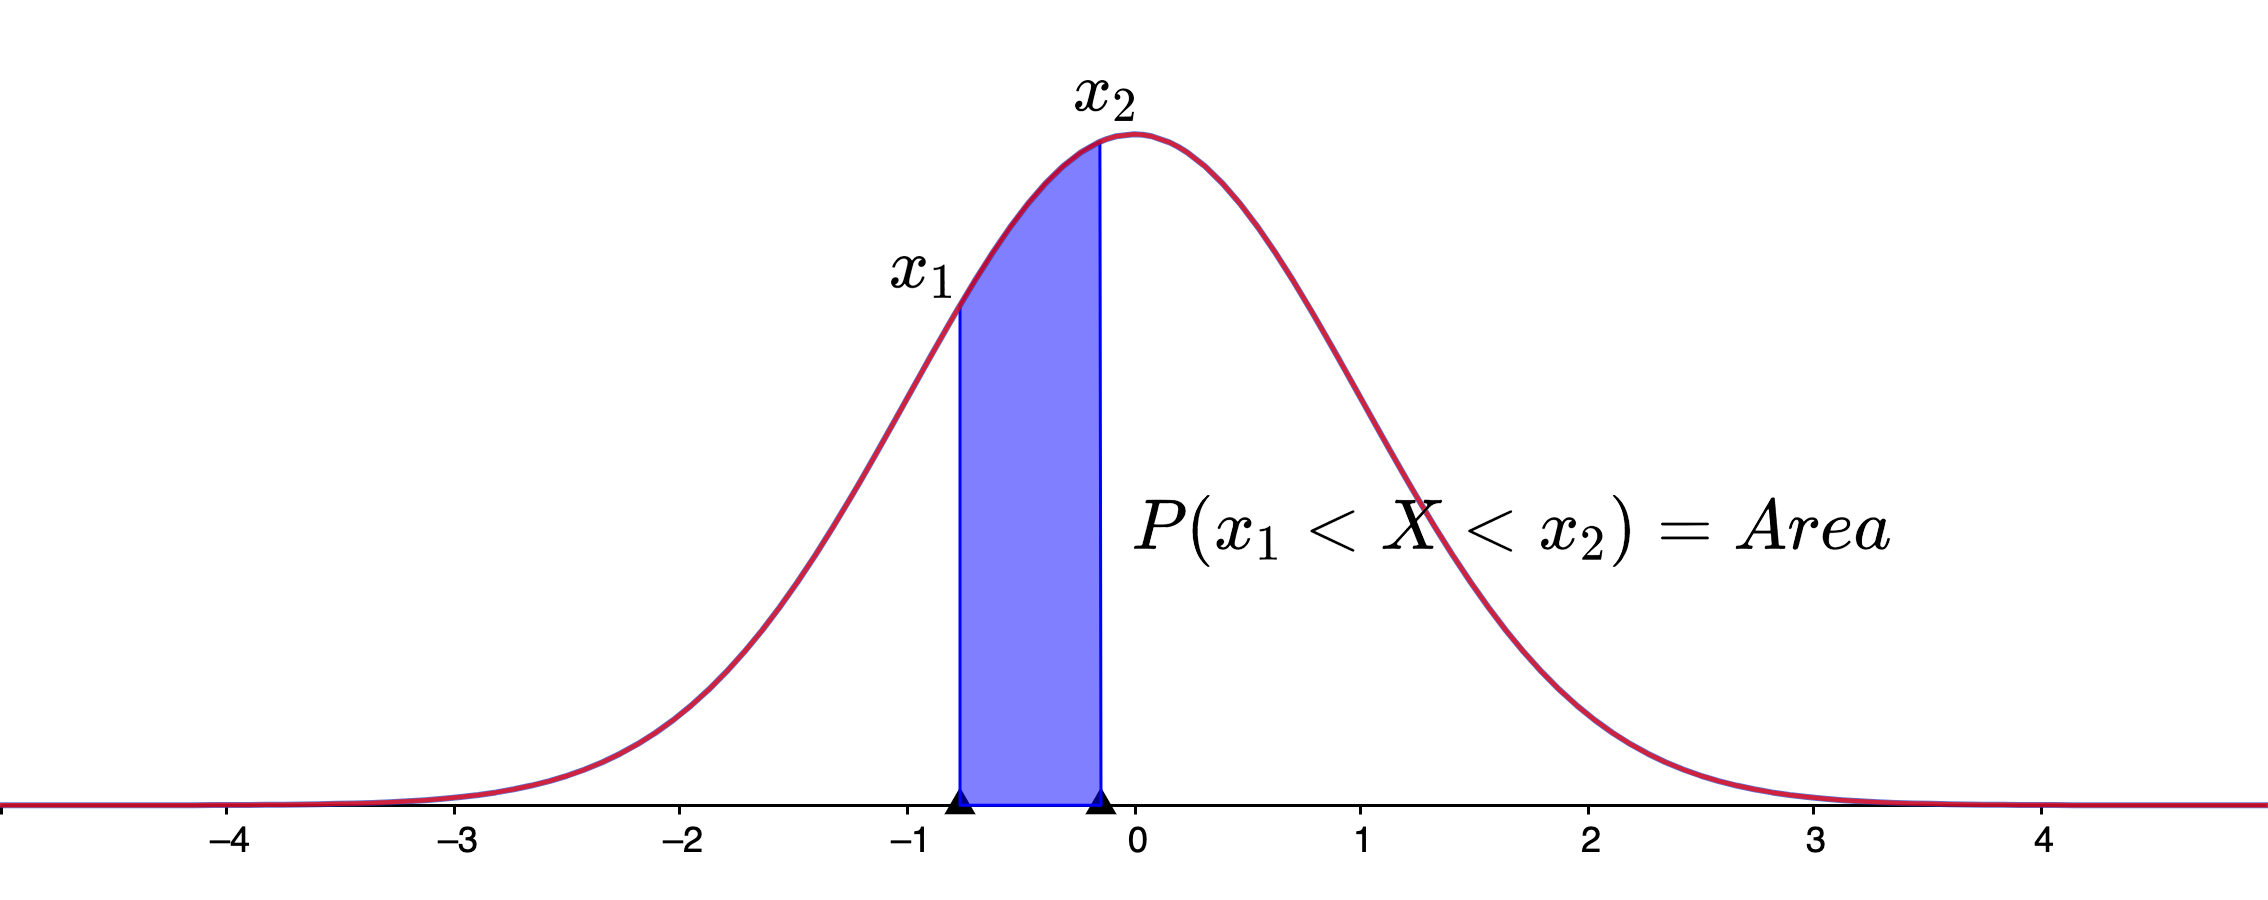
\includegraphics[width=0.8\textwidth]{Probability}
\caption{利用正态分布曲线查询概率}
\end{figure}
通过这种迂回手段,我们就变相地可以得到正态分布情况下的概率表了。这也是为什么之前图像当中,婴儿的质量采用了分段质量的一个原因。

\subsubsection*{正态分布的几种概率类型}
因此在求算正态分布的时候,有以下的三种类型,分别对应着以下的三类图像。
\begin{figure}[H]
\centering
\includegraphics[width=0.3\textwidth]{type1}
\includegraphics[width=0.3\textwidth]{type2}
\includegraphics[width=0.3\textwidth]{type3}
\end{figure}
他们分别对应着$P(X<z_1)$, $P(z_1<X<z_2)$, $P(X>z_1)$这三种概率。

\subsubsection*{1倍,2倍,3倍}
\label{subsub:3sd}
可以尝试点击\href{https://www.desmos.com/calculator/q8piat9t0t}{desmos链接}。任意调整期望和标准差,利用desmos当中CDF功能,求算$P(\mu-1\sigma<x<\mu+1\sigma)$,$P(\mu-2\sigma<x<\mu+2\sigma)$和$P(\mu-3\sigma<x<\mu+3\sigma)$的概率。

不同的同学会有不同的$\mu$和$\sigma$但是这三个概率是恒定值,分别是$0.68269$,$0.95449$和$0.99730$。因此,就得到如下的一张图表,表示随机变量的取值偏离该期望1倍,2倍,3倍标准差的时候的概率。如果简单用百分数表示的话,分别是1倍标准差以内概率为$68\%$,2倍标准差以内概率为$95\%$,3倍标准差以内概率为$99\%$。

\begin{figure}[H]
\centering
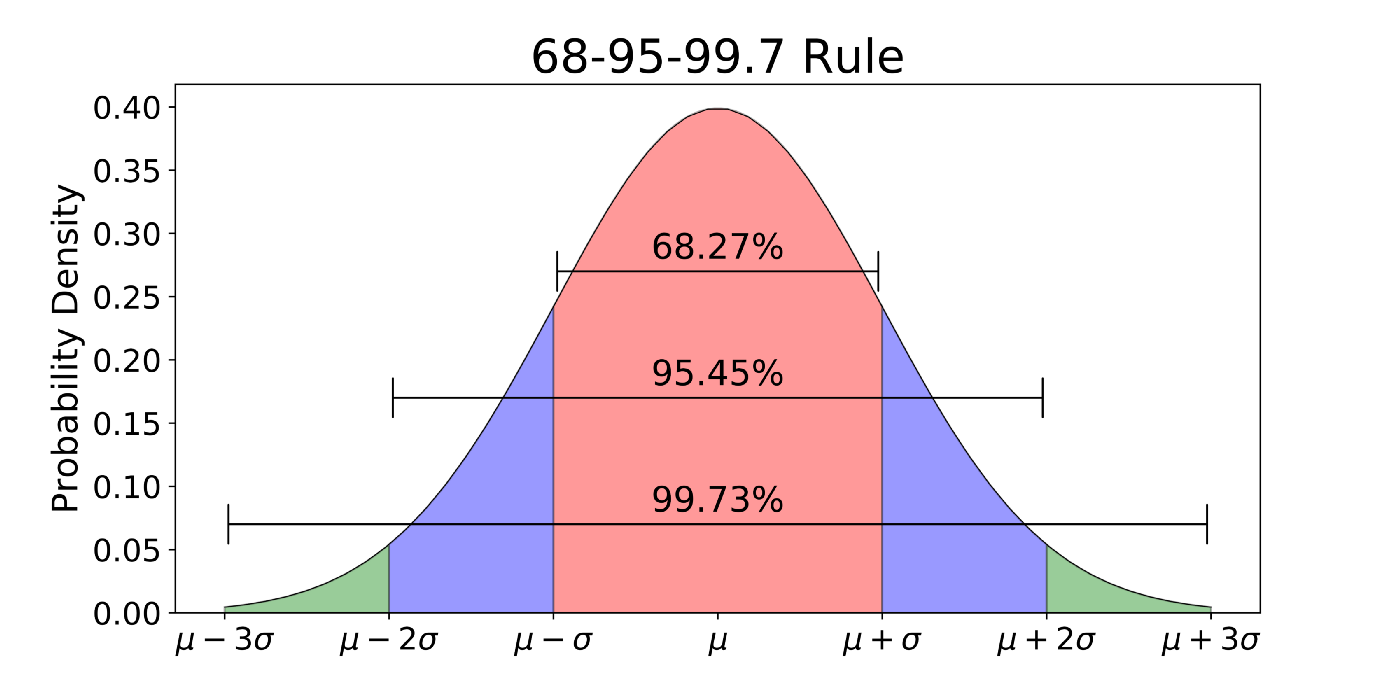
\includegraphics[width=0.8\textwidth]{3sd}
\caption{1倍,2倍,3倍标准区间内的概率}
\end{figure}

这个点在S2的部分将会不停地重复,不过在这里并不需要掌握。不过我借用这个表格来提出一个疑问。

如果使用某一个正态分布作为最基本的标杆(或者货币上的曲线),这个正态分布的期望和标准差应该是多少?

\subsubsection*{标准正态分布表}
上一个小节的答案绝大多数可能都会选择,$\mu=0$,$\sigma=1$。因为无论从表达式还是图像的角度,这个$N(0,1^2)$作为标杆是再合适不过的。这个分布就被称之为\gls{snd},有的时候也被计作$z-$distribution。所以,在当年没有计算器的情况下,另一个神——拉普拉斯计算了$\int_{-\infty}^x e^{-t^2} \d t$的积分表。Kramp站在他的肩膀上完成了标准正态分布表。也是考试MF19公式表里第10页的表格。

截取如下:
\begin{figure}[H]
\centering
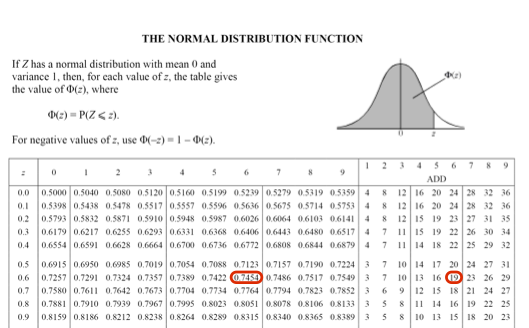
\includegraphics[width=0.8\textwidth]{normaltable}
\end{figure}

首先,这个表格的右上方是正态分布表格,阴影部分的面积显然代表随机变量$Z<z$值的概率。因此也就是表格当中的主体部分的取值。不过为了方便,我们用大写字母$\Phi$来表示累积概率。因此有:
\[
	\Phi(z)=P(Z<z)=\int_{-\infty}^{z} \phi(x) \d x = Area
\]
中间的积分不认识也没有关系,只需要理解用面积代表随机变量$Z<z$的概率就可以。

好,现在开始查表。如果需要查询$P(Z<0.666)$的概率的话,首先,先看主表的竖排,找到$0.6$的那一行,接下来再沿着横向找$6$的地方(主表当中的横排$0-9$代表的是百分位上的数值)。因此找到概率值为$0.7454$。注意,此时还没有结束,此时我们其实求算了$P(Z<0.660)$。还有千分位上的$6$需要确定,因此需要看附表ADD。附表当中的$1-9$就是千分位上的值,找到$6$,对应需要的增加量为$19$.意味着最终概率结果为$0.7454+0.0019=0.7473$。这就是完整的已知$z$值,查询概率的过程。

考试当中还有一种考察方式是给定概率,如$\Phi(z)=P(Z<z)=0.8392$,反求$z$的值这种逆向过程的题目。答案为$x=0.991$。

第三种考察方式是利用对称性,得到的$\Phi(-x) = 1-\Phi(x)$这样的公式,比如求算$P(x<-0.666)$。由于该正态分布表并没有展示$z$为负值的时候的结果,但是根据对称性,不难发现左侧的面积和右侧的面积关于$z=0$对称且相等。因此$\Phi(-0.666)=1-\Phi(0.666)=0.2527$

第四种考察方式是求算$P(z_1<Z<z_2)$。利用的公式为$\Phi(z_2)-\Phi(z_1)$。比如求算$P(-0.666<Z<0.666)$。利用该结论,最终结果为$0.7473-0.2527=0.4946$
以上的四种查询都需要掌握,尤其是千万区分清楚哪个是$z$值,哪个是概率$P(Z<z)$。在\ref{sec:classic problem}部分,进行实际题目的求算

\subsubsection*{标准化}
其实本可以不用写这个章节的内容,但是由于A-Level考试当中不允许使用可以求算任意正态概率的计算器。必须考察学生利用标准正态分布表求解标准正态分布的问题。因此需要掌握将任意一个$X\sim N(\mu,\sigma)$通过\gls{standardize}的手段转变为z-distribution,再查表解决问题。这也是\ref{subsub:3sd}中,为什么随便调整$\mu$,$\sigma$,63-95-97rule能成立的原因。

如果一个随机变量$X\sim  N(\mu,\sigma)$。那么将该随机变量减去其期望,再除以标准差之后得到的新随机变量$Z$必然满足标准正态分布。用公式来说明就是
\[
	Z\sim N(0,1^2),\quad Z=\frac{X-\mu}{\sigma} 
\]

\begin{ExampleBox}
已知$X\sim N(9,2^2)$,求算$P(X<10)$的概率。
\tcblower
做标准化之后$Z=\frac{X-9}{2^2}$。因此$P(X<10)=P(Z<\frac{10-9}{2})$。查询标准正态分布表$z=0.5$得到结果为$0.6919$。
\end{ExampleBox}

\subsection*{正态分布预估二项分布}
现在回过头再看看\ref{fig:binomial graph},像不像一个正态分布图?如果是的话,这个正态分布的期望和标准差分别是多少呢?

这一小节的标题,也就知道了,必然是像的。并且,这个正态分布的期望就是原来二项分布的均值,标准差也必定和二项分布的标准差一致。

\begin{ExampleBox}
如果$X\sim B(20,0.5)$, $\mu = E(X)=np=10$, $\sigma = \sqrt{Var(X)}=\sqrt{np(1-p)}=\sqrt{5}$。

因此$X\sim N(10,\sqrt{5}^2)$
\end{ExampleBox}

\subsubsection*{能够预估的条件}
该考点无需证明,只需要了解,当一个二项分布$B(n,p)$满足以下条件时:
\[
	np>5,\qquad  nq = n(1-p)>5
\]
就可以认为该二项分布近似于一个正态分布\footnote{在北美体系下,一般选择10} $N(np,\sqrt{np(1-p)}^2)$。如果感兴趣的话可以点击\href{http://bcs.whfreeman.com/webpub/Statistics/tps3e/Statistical_Applets/clt-binomial.html}{中心极限定理}了解更多

\subsubsection*{Continuity Correction}
因此当我们利用$N(10,\sqrt{5}^2)$来预估$P(X=10)$的话,会出现一个问题,就是正态分布是连续型的,但是二项分布是离散型的,也就意味着,需要用正态分布的区间概率来估计。而这个区间该取多少呢?其实在二项分布的图像当中我们已经讨论到这个事情了,$[9.5,10.5]$是二项分布柱状图的区间跨度,那么在正态分布当中也是使用这个区间。所以有:
\[
	P(X_B=10) = P(9.5<X_N<10.5) 
\]
因此,预估的结果为$\Phi (\frac{10.5-10}{\sqrt 5})-\Phi (\frac{9.5-10}{\sqrt 5})=0.1769$。而使用二项分布计算的结果为$\binom{20}{10}\cdot 0.5^10\cdot (1-0.5)^10=0.1762$。两者之间存有一定的误差,但是在可接受的范围内。

这种把离散值的随机变量变成连续值的过程就是连续性修正。对于这一类用正态分布预估二项分布的共有$7$种连续性修正。

\begin{table}[H]
\centering
\begin{tblr}{
	colspec={|c|[2pt]c|},
	hspan=even, %设置一样长度
	vspan=even,
	}
\hline 
Discrete Variable & Continuous Variable \\
\hline
$X=c$ & $c-0.5<X<c+0.5$\\ \hline
$X<c$ & $X<c-0.5$\\ \hline
$X\leqslant c$ & $X<c+0.5$\\ \hline
$X>c$ & $X>c+0.5$\\ \hline
$X\geqslant c$ & $X\geqslant c+0.5$\\ \hline
$c_1<X<c_2$ & $c_1+0.5<X<c_2-0.5$\\ \hline
$c_1\leqslant X\leqslant c_2$ & $c-0.5<X<c+0.5$ \hline
\end{tblr}
\end{table}

不需要记忆,去画二项分布的柱状图。然后理解什么样的时候会包含就可以了。
\clearpage

\section{经典例题}
\label{sec:classic problem}
下面就是这一章节的几条典型例题,如果都能够做一遍,并且完成的话这一章节就绝对没有问题了。





